%%%%%%%%%%%%%%%%%%%%%%%%%%%%%%%%%%%%%%%%%
% Journal Article
% LaTeX Template
% Version EG-1.6 (10/07/2018)
%
% This template is a modified version of a template downloaded from
% http://www.LaTeXTemplates.com, originally created by Frits Wenneker
% (http://www.howtotex.com) with extensive modifications by Vel
% (vel@LaTeXTemplates.com).
%
% This version further modified by Eduard Grebe (ed@eduardgrebe.net). A few
% elements of the PLOS submission style have been incorporated
%
% Available from https://github.com/eduardgrebe/preprint-latex-template
%
% License:
% CC BY-NC-SA 3.0 (http://creativecommons.org/licenses/by-nc-sa/3.0/)
%
% This template is designed to be compiled with XeLaTeX
%
%%%%%%%%%%%%%%%%%%%%%%%%%%%%%%%%%%%%%%%%%

%----------------------------------------------------------------------------------------
%	PACKAGES AND OTHER DOCUMENT CONFIGURATIONS
%----------------------------------------------------------------------------------------

\documentclass[a4paper,12pt,british]{article} %twocolumn 12pt
\usepackage[british]{babel} % Language hyphenation and typographical rules
\usepackage[hmarginratio=1:1,top=32mm,columnsep=20pt,headheight=15pt]{geometry} % Document margins

\usepackage{blindtext} % Package to generate dummy text throughout this template

% Uncomment the following 3 lines for compilation with pdflatex
%\usepackage[sc]{mathpazo} % Use the Palatino font
%\usepackage[T1]{fontenc} % Use 8-bit encoding that has 256 glyphs
%\usepackage[utf8]{inputenc}

% The next 3 lines require compilation with XeLaTeX and installation of
% Baskerville and Menlo (default on macOS). To compile with pdflatex comment out
% these lines and uncomment the mathpazo lines
\usepackage{fontspec} % \usepackage[no-math]{fontspec}
\setmainfont[Mapping=tex-text]{Baskerville}
\setmonofont[Scale=0.8]{Menlo}


% This should use a maths font that matches Palatino
%\usepackage{mathpazo}
%\linespread{1.05} % Line spacing - Palatino needs more space between lines
%\usepackage{microtype} % Slightly tweak font spacing for aesthetics

% Maths
\usepackage{amsmath}

% The next 3 lines require compilation with XeLaTeX and installation of
% Baskerville and Menlo (default on macOS). To compile with pdflatex comment out
% these lines and uncomment the mathpazo line
\usepackage{unicode-math}
\unimathsetup{math-style=TeX} % set to ISO if you desire upright capital Greek letters
\setmathfont{Asana-Math.otf}


\usepackage[center,labelfont=bf,up,textfont=bf,up]{caption} % Custom captions under/above floats in tables or figures
\usepackage{booktabs} % Horizontal rules in tables

\usepackage{lettrine} % The lettrine is the first enlarged letter at the beginning of the text

\usepackage{enumitem} % Customized lists
\setlist[itemize]{noitemsep} % Make itemize lists more compact

\usepackage{abstract} % Allows abstract customization
\renewcommand{\abstractnamefont}{\normalfont\bfseries\large} % Set the "Abstract" text to bold
\renewcommand{\abstracttextfont}{\normalfont\normalsize} % Set the abstract itself to small italic text %\small\itshape

\usepackage{titlesec} % Allows customization of titles
%\renewcommand\thesection{\Roman{section}} % Roman numerals for the sections
%\renewcommand\thesubsection{\roman{subsection}} % roman numerals for subsections
%\titleformat{\section}[block]{\large\scshape\centering}{\thesection.}{1em}{} % Change the look of the section titles
%\titleformat{\subsection}[block]{\large}{\thesubsection.}{1em}{} % Change the look of the section titles

\usepackage[calc]{datetime2} %Dates in ISO format
  \DTMnewdatestyle
    {dMyyyy}% label
    {% definitions
      \renewcommand*{\DTMdisplaydate}[4]{
      \number##3
      \space
      \DTMmonthname{##2}
      \number##1}
      \renewcommand*{\DTMDisplaydate}{\DTMdisplaydate}
    }
    \DTMnewdatestyle
      {Myyyy}% label
      {% definitions
        \renewcommand*{\DTMdisplaydate}[4]{
        \DTMmonthname{##2}
        \number##1}
        \renewcommand*{\DTMDisplaydate}{\DTMdisplaydate}
      }

  %\DTMsetdatestyle{Myyyy} % Set date display to, e.g. "July 2018"
  \DTMsetdatestyle{dMyyyy} % Set date display to, e.g. "6 July 2018"

%\usepackage{fancyhdr} % Headers and footers
%\pagestyle{fancy} % All pages have headers and footers
%\fancyhead{} % Blank out the default header
%\fancyfoot{} % Blank out the default footer
%\fancyhead[C]{Performance comparison Maxim and Sedia LAg $\bullet$ \Today} % Custom header text % $\bullet$ Vol. XXI, No. 1
%\fancyfoot[C]{\thepage} % Custom footer text

\usepackage{titling} % Customizing the title section

\usepackage{authblk}
\renewcommand\Affilfont{\footnotesize}

\usepackage{hyperref} % For hyperlinks in the PDF

% Use adjustwidth environment to exceed column width (see example table in text)
\usepackage{changepage}

\usepackage{graphicx}

%\usepackage{array}
% \thickhline command for thick horizontal lines that span the table
%\newcommand\thickhline{\noalign{\global\savedwidth\arrayrulewidth\global\arrayrulewidth 2pt}%
%\hline
%\noalign{\global\arrayrulewidth\savedwidth}}



%----------------------------------------------------------------------------------------
%	TITLE SECTION
%----------------------------------------------------------------------------------------

\setlength{\droptitle}{-4\baselineskip} % Move the title up

\pretitle{\begin{center}\Huge\bfseries} % Article title formatting
\posttitle{\end{center}} % Article title closing formatting

\title{Article Title} % Article title

\author[1†*]{Eduard Grebe}
\author[2†]{Second Author}
\author[3]{Third Author}
\affil[1]{DST-NRF Centre of Excellence in Epidemiological Modelling and Analysis (SACEMA), Stellenbosch University, Stellenbosch, South Africa}
\affil[2]{Second Affiliation}
\affil[3]{Third Affiliation}
\affil[†]{These authors contributed equally.}
\affil[*]{\href{mailto:eduardgrebe@sun.ac.za}{eduardgrebe@sun.ac.za}}
\date{\Today} % Leave empty to omit a date
\renewcommand{\maketitlehookd}{%
\begin{abstract}
\noindent \blindtext % Dummy abstract text - replace \blindtext with your abstract text
\end{abstract}
}

%----------------------------------------------------------------------------------------

\begin{document}

% Print the title
\maketitle

%----------------------------------------------------------------------------------------
%	ARTICLE CONTENTS
%----------------------------------------------------------------------------------------

\section{Introduction}

\lettrine[nindent=0em,lines=3]{L} orem ipsum dolor sit amet, consectetur adipiscing elit.
\blindtext % Dummy text

\begin{eqnarray}
\label{eq:kassanjee}
\lambda = \frac{P_H \cdot (P_{R|+}-\epsilon_T)}{(1 - P_H) \cdot (\Omega_T - \epsilon_T \cdot T)}
\end{eqnarray}

\blindtext % Dummy text

%------------------------------------------------

\section{Methods}

Maecenas sed ultricies felis. Sed imperdiet dictum arcu a egestas.
\begin{itemize}
\item Donec dolor arcu, rutrum id molestie in, viverra sed diam
\item Curabitur feugiat
\item turpis sed auctor facilisis
\item arcu eros accumsan lorem, at posuere mi diam sit amet tortor
\item Fusce fermentum, mi sit amet euismod rutrum
\item sem lorem molestie diam, iaculis aliquet sapien tortor non nisi
\item Pellentesque bibendum pretium aliquet
\end{itemize}
\blindtext % Dummy text

Text requiring further explanation\footnote{Example footnote}.

%------------------------------------------------

\section{Results}

In the results section we have Table~\ref{table1} and Table~\ref{table2}.

\begin{table}
\centering
\caption{Example table}
\begin{tabular}{llr}
\toprule
\multicolumn{2}{c}{Name} \\
\cmidrule(r){1-2}
First name & Last Name & Grade \\
\midrule
John & Doe & $7.5$ \\
Richard & Miles & $2$ \\
\bottomrule
\end{tabular}
\label{table1}
\end{table}

\begin{table} %[!ht] uncomment to control placement
\caption{‘Average incidence’ estimates by age group using the biomarker and synthetic cohort methods}
\centering
\resizebox{\textwidth}{!}{%
\begin{tabular}{|l|c|c|c|c|c|c|}
\hline
                                      & \multicolumn{3}{|c|}{\bf Age-continuous biomarker mothod} & \multicolumn{3}{|c|}{\bf Synthetic cohort method}    \\ \hline
\multicolumn{1}{|c|}{\bf Age group}   & {\bf Males}         & {\bf Females}       & {\bf Total}         & {\bf Males}         & {\bf Females}       & {\bf Total} \\
                                      & P.E. (95\% CI)      & P.E. (95\% CI)      & P.E. (95\% CI)      & P.E. (95\% CI)      & P.E. (95\% CI)      & P.E. (95\% CI) \\
\multicolumn{1}{|c|}{\emph{years}}    & \emph{cases/100PY}  & \emph{cases/100PY}  & \emph{cases/100PY}  & \emph{cases/100PY}  & \emph{cases/100PY}  & \emph{cases/100PY} \\ \hline %\thickhline
[15,20)                               & 0.45 (0.08,0.88)    & 1.92 (1.02,3.05)    & 1.20 (0.73,1.78)    & 0.27 (0.00,0.60)    & 2.90 (2.30,3.48)    & 1.61 (1.24,1.92) \\ \hline
[20,25)                               & 0.71 (0.16,1.38)    & 3.73 (2.41,5.30)    & 2.20 (1.51,2.92)    & 1.59 (1.14,2.05)    & 5.26 (4.53,6.20)    & 3.40 (2.96,3.91) \\ \hline
[25,30)                               & 1.50 (0.40,2.73)    & 3.62 (2.04,5.38)    & 2.52 (1.52,3.45)    & 5.09 (3.36,6.64)    & 5.70 (4.33,7.30)    & 5.38 (4.23,6.65) \\ \hline
[30,35)                               & 2.02 (0.24,4.50)    & 2.66 (0.71,5.47)    & 2.33 (0.99,4.30)    & 4.07 (0.00,11.18)   & 8.53 (2.29,16.43)   & 6.20 (2.47,11.29) \\ \hline
[15,30)                               & 0.81 (0.22,1.45)    & 2.95 (1.98,4.04)    & 1.87 (1.31,2.43)    & 2.00 (1.53,2.46)    & 4.39 (4.00,4.85)    & 3.19 (2.83,3.56) \\ \hline
\end{tabular}
}
\label{table2}
\end{table}

\blindtext

We also have Figure~\ref{figure1}. We can calso refer explicitly to equations, for example Equation~\ref{eq:emc}

\begin{figure}[!h] % here we are forcing placement
\caption{HIV incidence by age in males and females aged 15-30, using the synthetic cohort, recency biomarker and combined methods.}
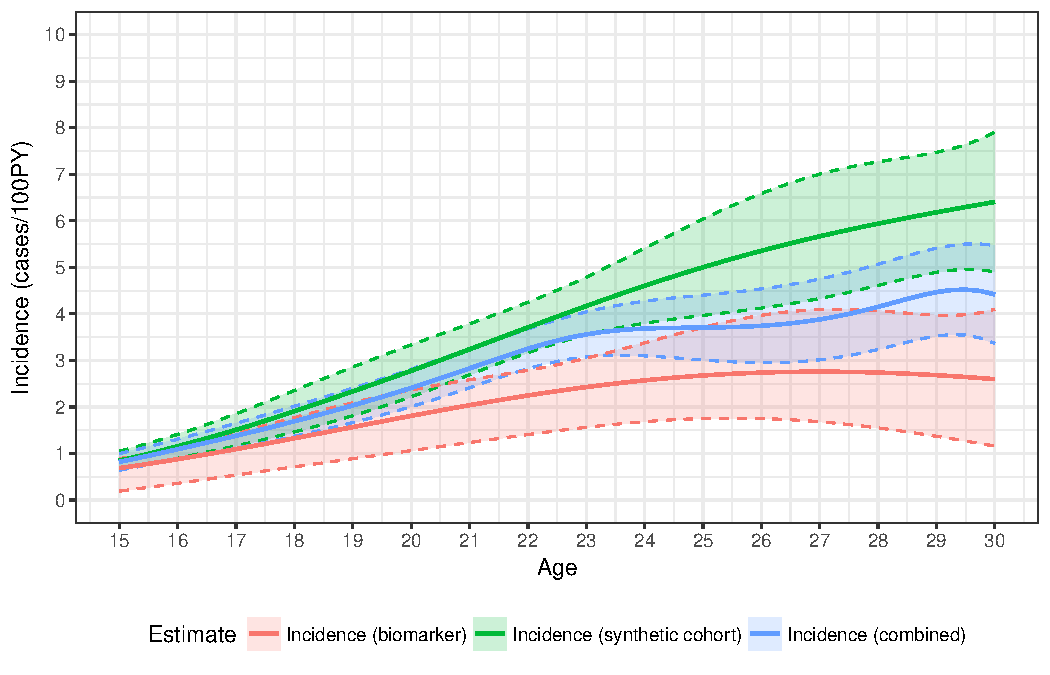
\includegraphics[width = 1\textwidth]{Figure1.pdf}
\label{figure1}
\end{figure}

\blindtext % Dummy text

\begin{equation}
\label{eq:emc}
e = mc^2
\end{equation}

\blindtext % Dummy text

%------------------------------------------------

\section{Discussion}

\subsection{Subsection One}

A statement requiring citation \cite{Schlegel2016} and another \cite{Williams2001}.

\blindtext % Dummy text

\subsection{Subsection Two}

\blindtext % Dummy text

%----------------------------------------------------------------------------------------
%	REFERENCE LIST
%----------------------------------------------------------------------------------------

\bibliography{references}

\bibliographystyle{plos2015}



%----------------------------------------------------------------------------------------

\end{document}
